\stepcounter{mysection}\section{\arabic{mysection} Основная часть}
	В первую очередь следует отметить тот весьма важный факт, что при работе над документом в \LaTeX создаётся проект
	с файлами разного типа, распределённых по поддиректориям. После сборки этого проекта создаётся PDF-файл, который
	является результатом вёрстки документа.

	В рамках данной работы разработан законченный проект, который можно использовать в качестве шаблона и примера
	для оформления отчётов, документов с помощью системы \LaTeX.

	\subsection{Структура проекта}
		Проект включает в себя разные типы  файлов:
			\begin{itemize}
				\fontsize{0pt}{0pt}
				\setlength{\itemsep}{0pt}
				\item Файлы исходных данных, которые обычно имеют расширение ".tex"; 
				\item Файлы, являющееся дополнительными ресурсами;
				\item Хранящие правила верстки файлы, которые хранятся с расширением ".sty";
				\item Необходимые для сборки файлы;
				\item Файлы для журналирования и для прочего.
			\end{itemize}

			Tex-файлы представляют собой набранный текст, включающий в себя некоторые команды \LaTeX. Эти команды детально описаны
			в WIKI-учебнике. Один tex-файл может включать в себя другие такие же файлы, что позволяет структурировать и хранить 
			части документа в местах, угодных пользователю. Эти файлы могут быть сгруппированы по смыслу или по виду их 
			применения. Например, проще работать с файлами, когда все файлы с таблицами и основными главами находятся в
			разных местах. Белее того, такая организация может распространяться не только на tex-файлы.

			Такой принцип организации позволяет с лёгкостью управлять частями документа: включать, исключать, менять местами и многое другое.
			Таким образом работа с документом становится удобнее и понятнее. И используя утилиты операционной системы или возможности
			текстового редактора, можно без каких-либо трудностей использовать навигацию для ещё быстрой работы над проектом.

			Ниже представлена структура разработанного проекта, где в корне проекта находится основной файл doc.tex, который включает в себя
			ссылки на другие файлы, необходимые для сборки проекта.

			Многие дистрибутивы linux-подобных операционных систем позволяют посмотреть структуру проекта через утилиту \texttt{tree}: \\
			\texttt{\footnotesize arlyapov\ $@$ pc \sim/article: tree}
			\newpage
			\texttt{\footnotesize 
				.\\
				├── biblio.bib\\
				├── doc.aux\\
				├── doc.bbl\\
				├── doc.blg\\
				├── doceverypage.sty\\
				├── doc.log\\
				├── doc.pdf\\
				├── docrequires.sty\\
				├── docsecondpage.sty\\
				├── docsettings.sty\\
				├── doc.tex\\
				├── doc.toc\\
				├── kurreport.cls\\
				├── src\\
				│~~~├── conclusion.tex\\
				│~~~├── drawings.tex\\
				│~~~├── introduction.tex\\
				│~~~├── offer.tex\\
				│~~~├── pictures\\
				│~~~│~~~├── drawingp1.png\\
				│~~~│~~~├── drawingp2.png\\
				│~~~│~~~├── offerp1.png\\
				│~~~│~~~├── offerp2.png\\
				│~~~│~~~├── picturep1.png\\
				│~~~│~~~├── program.png\\
				│~~~│~~~├── projectp1.png\\
				│~~~│~~~├── schemep1.png\\
				│~~~│~~~├── schemep2.png\\
				│~~~│~~~└── schemep3.png\\
				│~~~├── picture.tex\\
				│~~~├── project.tex\\
				│~~~├── schemes.tex\\
				│~~~├── spec.tex\\
				│~~~├── tables\\
				│~~~│~~~├── offert1.tex\\
				│~~~│~~~├── offert2.tex\\
				│~~~│~~~├── offert3.tex\\
				│~~~│~~~├── projectt1.tex\\
				│~~~│~~~├── schemet1.tex\\
				│~~~│~~~├── taskt1.tex\\
				│~~~│~~~└── taskt2.tex\\
				│~~~└── task.tex\\
				└── title.tex 
			}

	\subsection{Титульный лист}
		Первое что включает в себя основной  tex-файл  в теле "document" - это ссылка на титульный лист. Сам же титульный лист оформлен в отдельном файле,
		обучающих материалов по работе с которым можно найти в различных книгах, WIKI-учебниках и видео.

		Оформление титульного листа происходит в блоке "titlepage", все описанные в нём правила верстки будут применены только к титульному листу. 
		И все необходимые исходные данные описываются в файле "title.tex".

	\subsection{Кастомизация}
		Следует уделить большое внимание файлам с правилами отображения. Если к документу нет большого количества требований, то достаточно описать
		необходимое в основном tex-файле перед телом "docuvent". В противном случае это нужно сделать в отдельном файле, а в основном указать ссылку на него.
		И это тоже не подойдёт в том случае, если к документу имеется большое количество требований и на описание правил в одном файле становится сложной задачей.

		
		Также следует отметить немаловажную вещь, в основном файле необходимо обозначить класс документа. Класс в себя включает уже определённые правила вёрстки,
		которые можно менять в соответствии с особенностями документа и пунктами в требованиях к документу.

		В данном проекте определён собственный класс "kurreport", который определён на основе класса "report". Файл используемый для определения пользовательского
		класса имеет одноимённое название и расширение "cls". И учитывая то, что описывать все правила в одном файле является непростой задачей, его содержимое разбито
		на четыре sty-файла. Файл\ "docrequires.sty"\ определяет зависимости от необходимых модулей системы; в файле\\ "docsettings.sty"\ описаны основные правила вёрстки
		для всего документа; а файлы\ "docsecondpage.sty"\ и "doceverypage.sty" необходимы для изображения рамок на второй и последующих страницах.
	\subsection{Рамка}

		На рисунке \ref{img1} отражены требования к рамке и основным надписям, которые необходимо соблюдать при оформлении отчётов.

		Как уже сказано выше, за оформление рамки отвечают файлы \\ "docsecondpage.sty"\ и "doceverypage.sty", в которых в тегах "AddEverypageHook"\ указаны
		необходимые настройки для добавления рамки и расположение надписей. Следует отметить, что нумерация и подсчёт количества страниц воспроизводится
		автоматически при том, что материал для этих страниц хранится в совершенно разных файлах.
			\begin{figure}[!htb]
				\minipage{0.5\textwidth}
					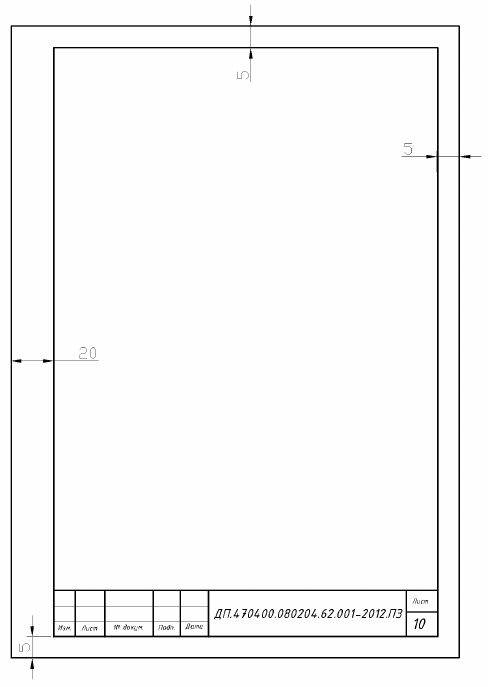
\includegraphics[width=\linewidth]{src/images/frame1.png}
					\centering
					Основная рамка
				\endminipage\hfill
				\minipage{0.5\textwidth}
					\centering
					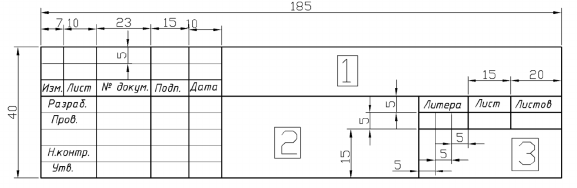
\includegraphics[width=\linewidth]{src/images/frame2.png}
					Основная надпись (второй лист)
					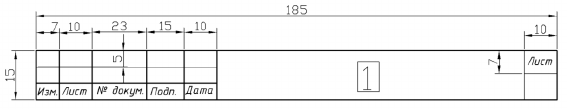
\includegraphics[width=\linewidth]{src/images/frame3.png}
					Основная надпись (последующие листы)
				\endminipage
				\caption{Рамка и основные надписи}\label{img1}
			\end{figure}

	\newpage
	\subsection{Ссылки и зависимости} % Автоматическиен списки
		Одним из самых главных приемуществ \LaTeX является то, что достаточно много вещей можно автоматизировать. Это касается и списка литература, который сам проставляет номера
		пунктов в списке относительно упоминания их в работе. Более того, если большая часть документа будет исключена, то нумерация и ссылки обновятся автоматически.
		И это применимо к оглавлению, таблицам, рисункам, нумерации глав и ссылок на всё перечисленное.

		А также есть возможность задавать пользовательский счётчик, который можно использовать одновременно практически везде. Всё это и остальное, описанное в WIKI-учебнике
		упрощает работу с проектом.
	\subsection{Дополнительные возможности}
		Ещё одни важный факт. Как уже говорилось выше, в процессе разработки проекта можно использовать систему контроля версий git, которая позволяет на базе одного проекта
		работать над целым перечнем документов. Принимая это во внимание, пользователь может заимствовать проделанную работу над одним документом для других на любом этапе разработки.
		А также это всё способствует командной разработке документов.
